%% This is an example first chapter.  You should put chapter/appendix that you
%% write into a separate file, and add a line \include{yourfilename} to
%% main.tex, where `yourfilename.tex' is the name of the chapter/appendix file.
%% You can process specific files by typing their names in at the 
%% \files=
%% prompt when you run the file main.tex through LaTeX.
\chapter{Analysis, Further Research Opportunities and Conclusion}

\section{Analysis}

\subsection{The Significance of Ensemble Size}

To observe the effect of ensemble size on the DSHEnKF filtering process, a 50 ensemble run and a 25 ensemble run were compared to the 100 ensemble run from chapter 4. The 50 ensemble and 25 ensemble run were identical to the 100 ensemble run in regards to starting parameters. Figure \ref{fig:194_ens} shows how streamflow estimations for an ungaged catchment in the filtering process evolve as more ensembles are added. As the leftmost graph demonstrates, small numbers of ensembles lead to spurious streamflow predictions in both the prior and posterior. However, as demonstrated in Figure \ref{fig:str194_UNGAGED}, this spurious behavior does not translate into the unfiltered run of the model. Figures \ref{fig:str194_UNGAGED} and \ref{fig:str_unfiltered} demonstrate how the model performs when utilizing the unfiltered 50 ensemble and 100 ensemble parameters.

\begin{figure}
\centering
\begin{minipage}{.33\textwidth}
  \centering
  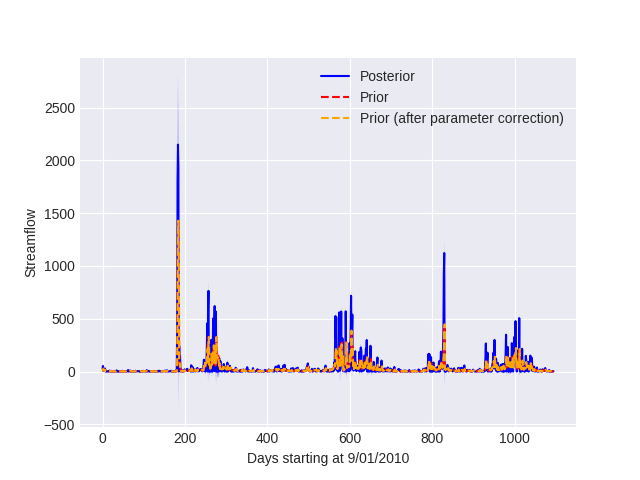
\includegraphics[width=.98\linewidth]{194_ens25}
  \label{fig:194_ens25}
\end{minipage}%
\begin{minipage}{.33\textwidth}
  \centering
  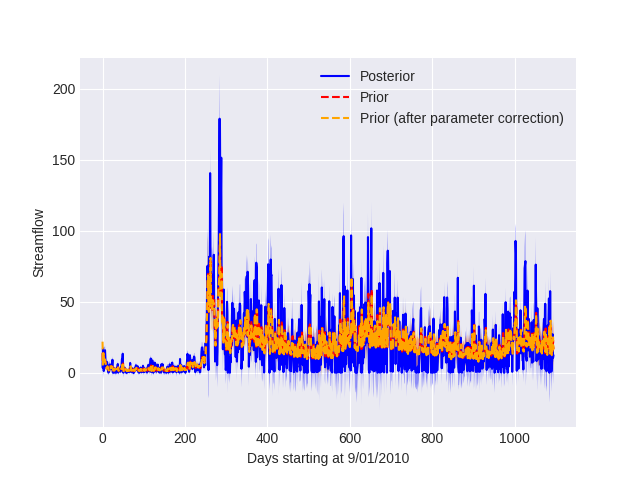
\includegraphics[width=.98\linewidth]{194_ens50}
  \label{fig:194_ens50}
\end{minipage}
\begin{minipage}{.33\textwidth}
  \centering
  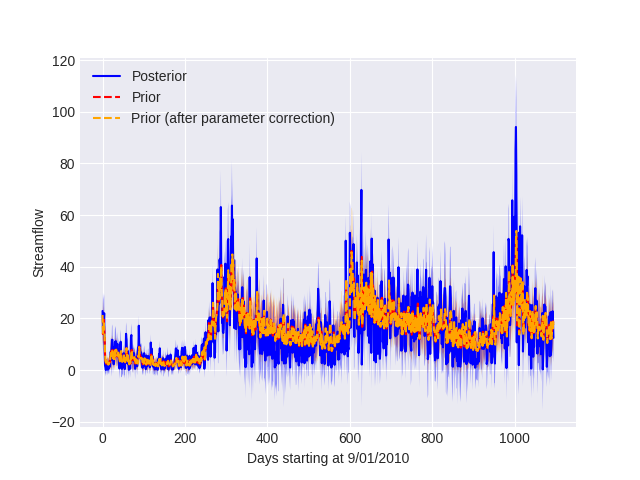
\includegraphics[width=.98\linewidth]{194_ens100}
  \label{fig:194_ens100}
\end{minipage}
\captionof{figure}{Streamflow states for ungaged catchment 194 during the filtering process. From left to right: 25 ensembles, 50 ensembles, 100 ensembles}
\label{fig:194_ens}
\end{figure}

\begin{figure}[h]
    \centering
    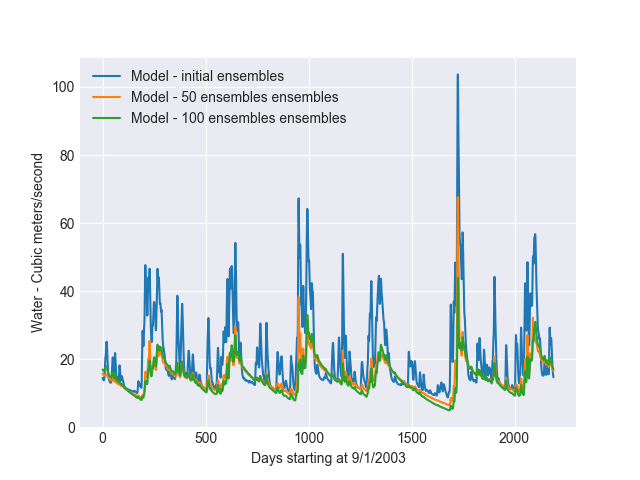
\includegraphics[width=0.95\textwidth]{str194_UNGAGED}
    \caption{The resulting hyrdologic model run over 6 years for the ungaged catchment 194 from Figure \ref{fig:194_ens}}
    \label{fig:str194_UNGAGED}
\end{figure}

\pagebreak

\subsection{Comparison of Filtered Parameters}

To analyze the accuracy of the Dual State Hierarchical Ensemble Kalman Filtering algorithm, the final calibrated parameter values were taken from Chapter 4's run and applied to a standard unfiltered hydrologic model. The model was run over a period of 6 years and the results were compared to a run of the hydrologic model with the initial parameters from Table 4.2, the 50 ensemble run mentioned earlier in this chapter, and the corresponding gauged catchments. Figure \ref{fig:str_unfiltered} shows the varying results from 4 catchments. Catchments 115 and 173 show a clear improvement over the initial modeled results. Catchment 173 demonstrates the danger of using an inferior number of ensembles, as the initial estimates are superior to the 50 ensemble run. Catchment 139 demonstrates a case where the filtered parameters were unable to successfully emulate the observed state. Overall, the filtered parameters represent an improvement over the non-filtered parameters when compared to the observed states.

\begin{figure}
\begin{tabular}{cc}

\subcaptionbox{Catchment 115\label{2}}{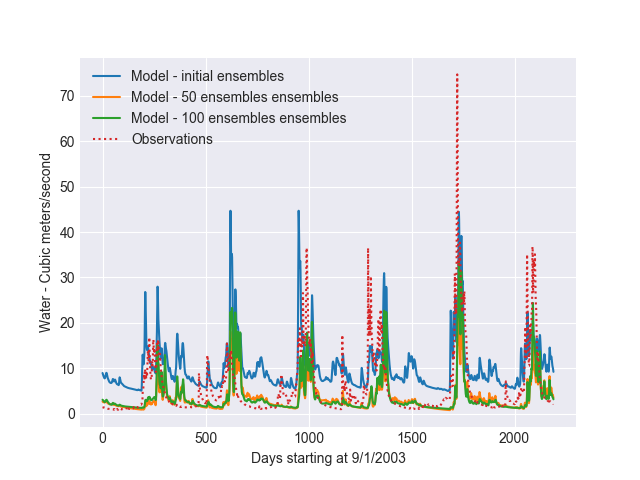
\includegraphics[width = .48\linewidth]{str115}} &
\subcaptionbox{Catchment 139\label{2}}{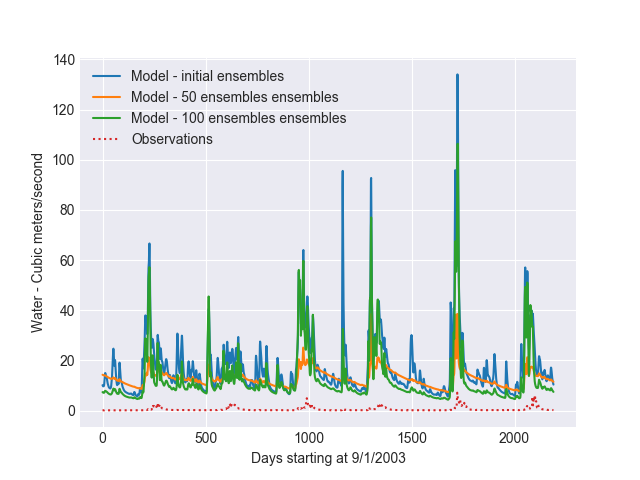
\includegraphics[width = .48\linewidth]{str139}}\\
\subcaptionbox{Catchment 165\label{2}}{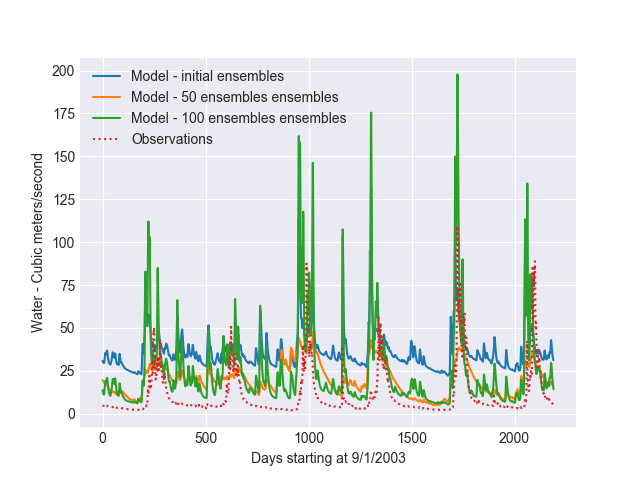
\includegraphics[width = .48\linewidth]{str165}} &
\subcaptionbox{Catchment 173\label{2}}{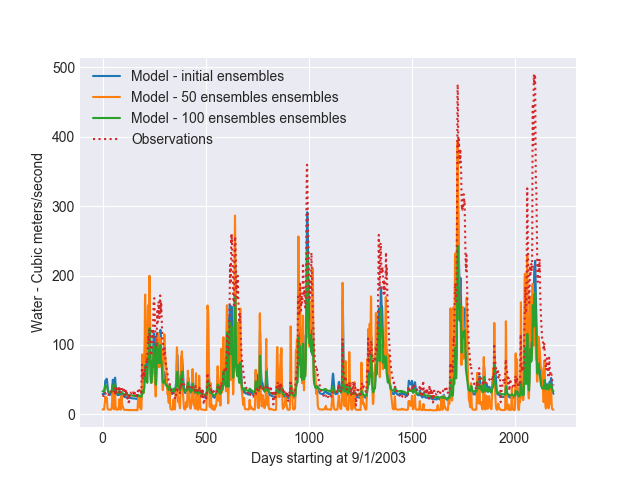
\includegraphics[width = .48\linewidth]{str173}}

\end{tabular}
\captionof{figure}{4 runs of the hydrologic model compared to the observed state: initial parameters from Table 4.2, parameters from a 50 ensemble run, parameters from a 100 ensemble run.}
\label{fig:str_unfiltered}
\end{figure}

\subsection{Groundwater Accumulation Process and Correlated Parameters}

While both the 50 ensemble run and 100 ensemble run of the model generally produced reasonably accurate streamflow estimates, many parameters, particularly the groundwater parameters \texttt{ck2} and \texttt{perc}, tended to differ greatly in spatial distribution. This warranted an evaluation of these parameter's correlation, the results of which can be seen in figure \ref{fig:correlatedck2perc}. \texttt{ck2} was determined to be inversely proportional to \texttt{perc}. Therefore, while these two parameters were calibrated in such a way that groundwater remained stable, different amounts of groundwater are collected and dispersed in the lower reservoir (Figure \ref{fig:str_unfiltered_gw}). Therefore, while the DSHEnKF placed all parameters in reasonable positions in both runs, the correlated nature of these and other parameters can result in different distributions of parameters. Correlated parameters have been documented in HBV models in the past \cite{Jakeman1993}, \cite{Merz2004}, \cite{Maneta2008} and as a result these results are not surprising and final parameters may be expected to lock onto new parameter values per each filtering run.

\begin{figure}[h]
    \centering
    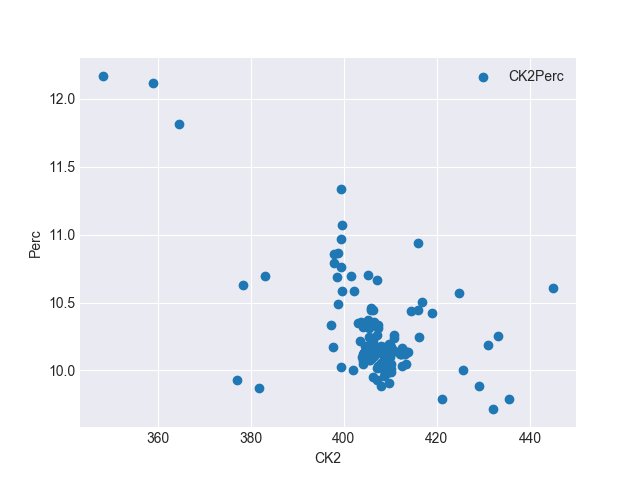
\includegraphics[width=0.95\textwidth]{correlatedck2perc}
    \caption{\texttt{perc} values plotted against \text{ck2} values.}
    \label{fig:correlatedck2perc}
\end{figure}

\begin{figure}
\begin{tabular}{cc}

\subcaptionbox{100 ensemble run: \texttt{ck2}\label{2}}{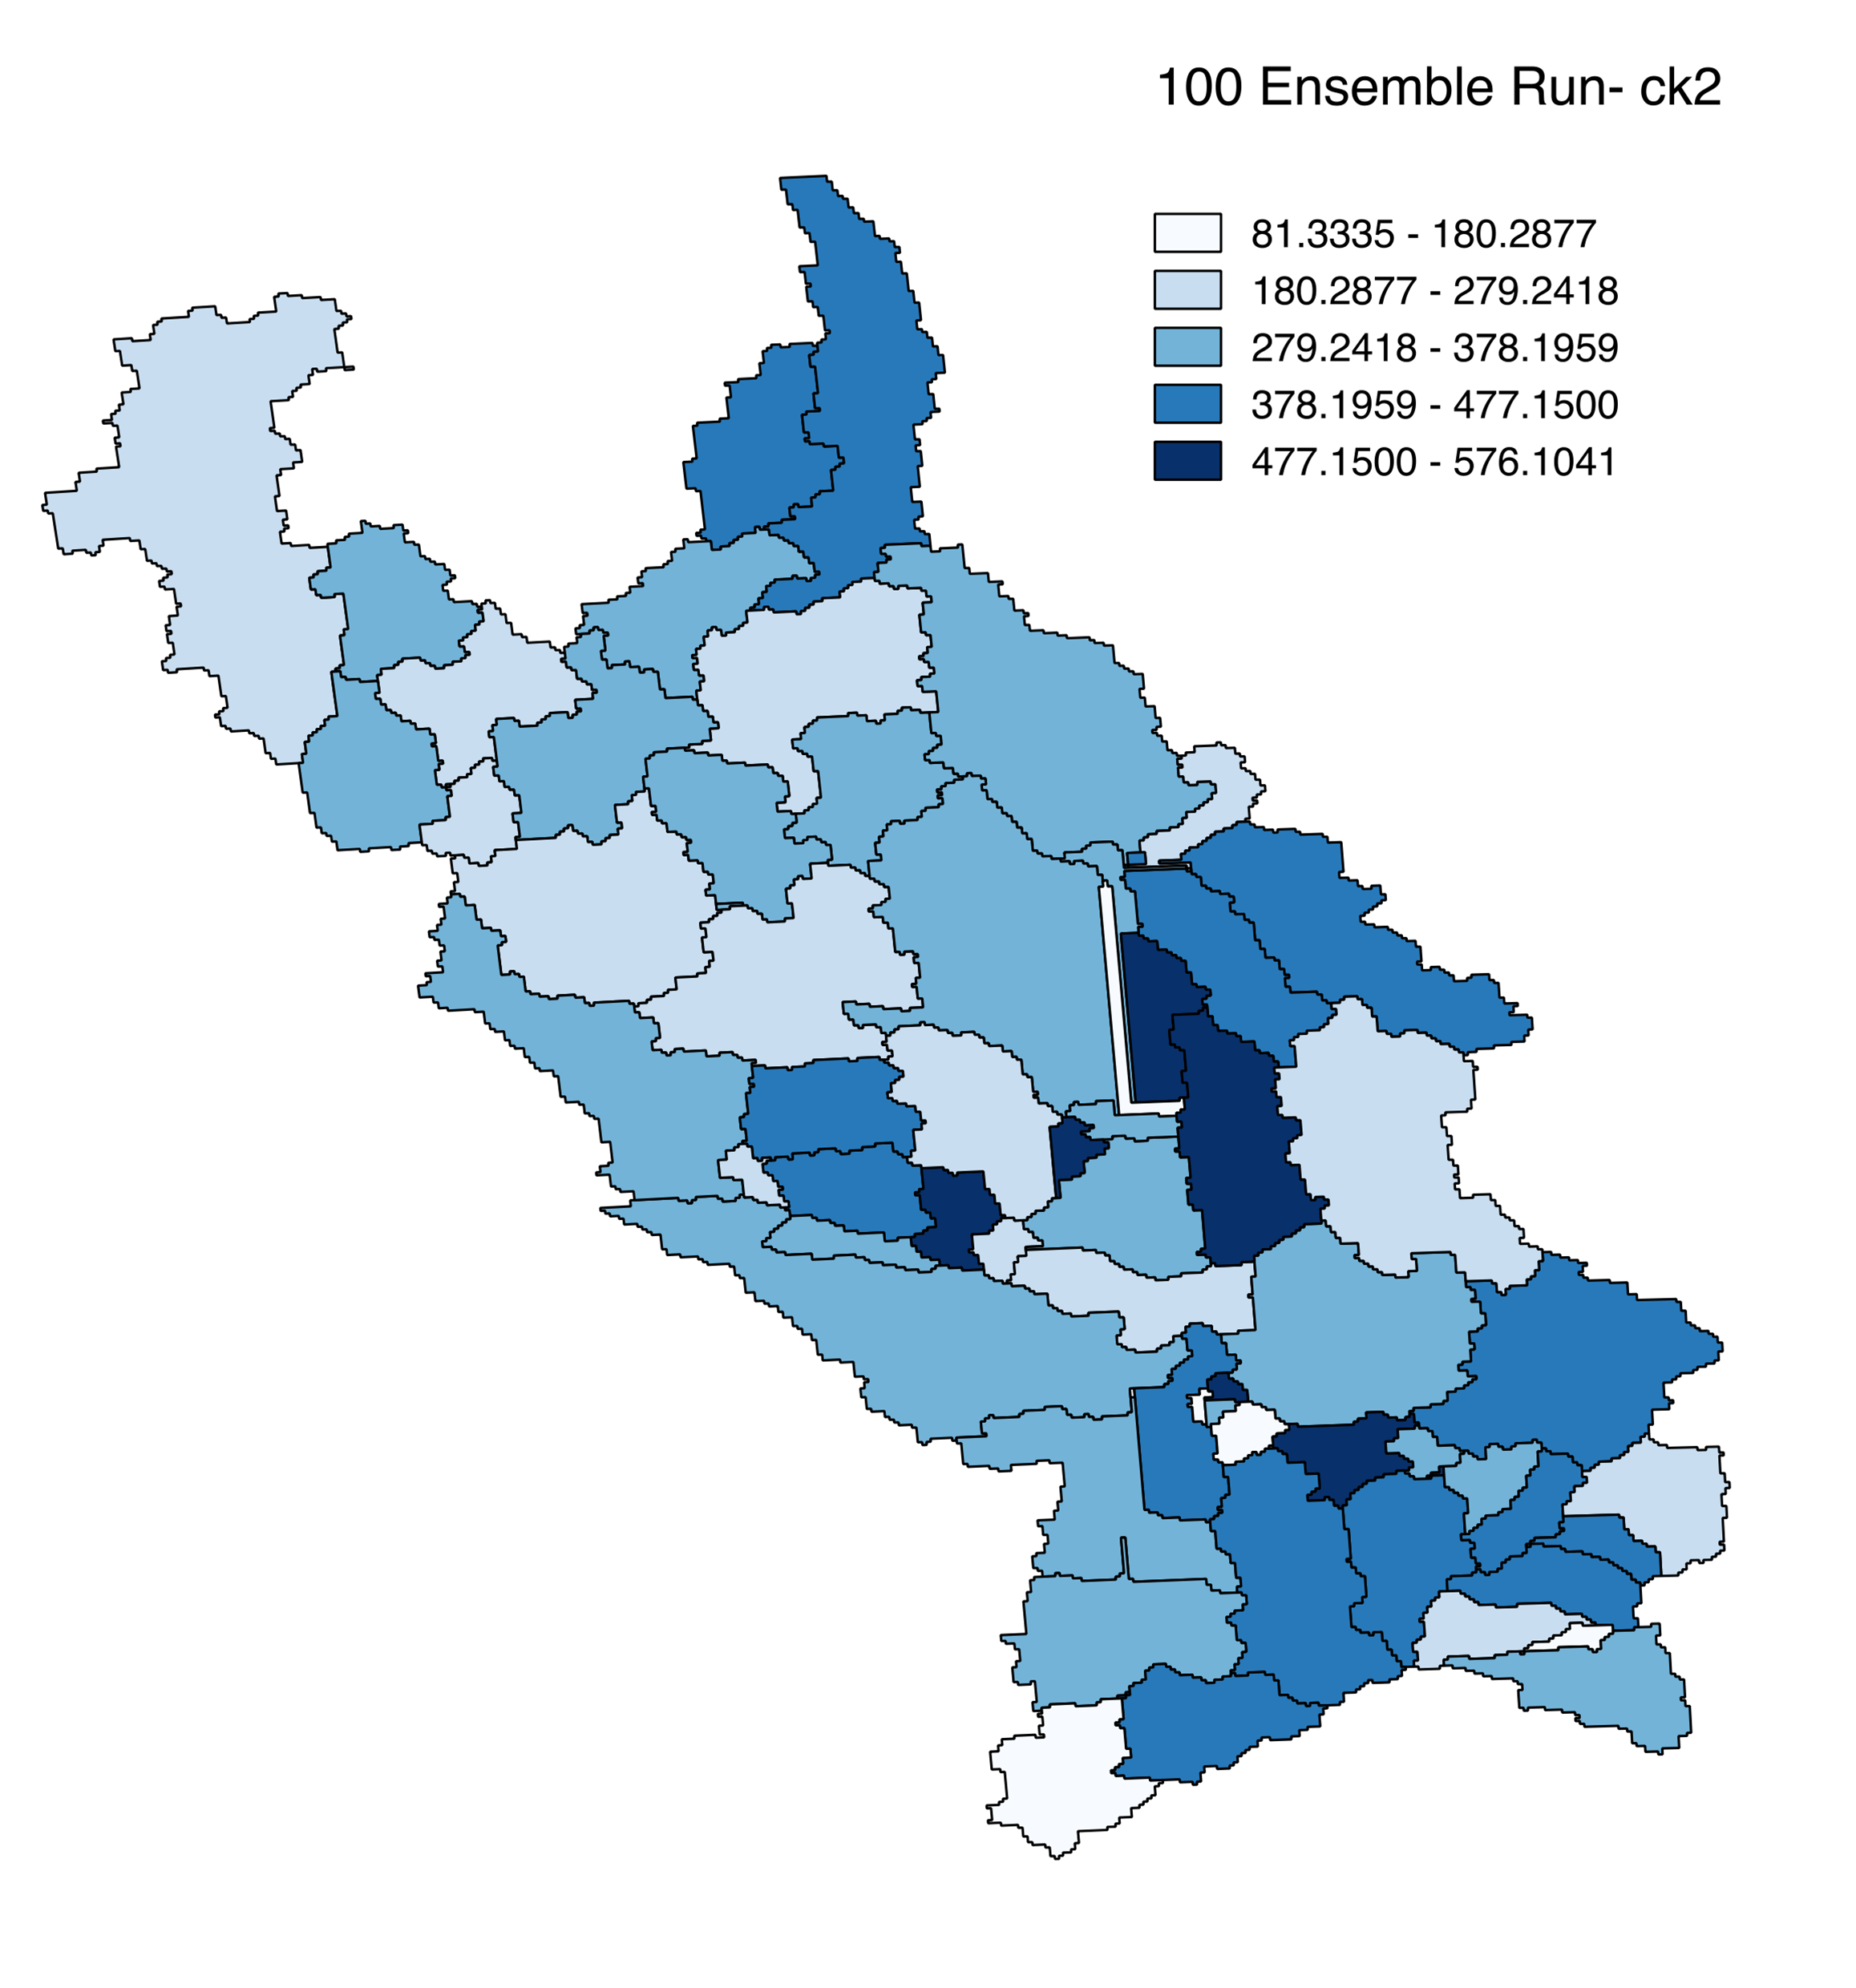
\includegraphics[width = .48\linewidth]{ck2100}} &
\subcaptionbox{50 ensemble run: \texttt{ck2}\label{2}}{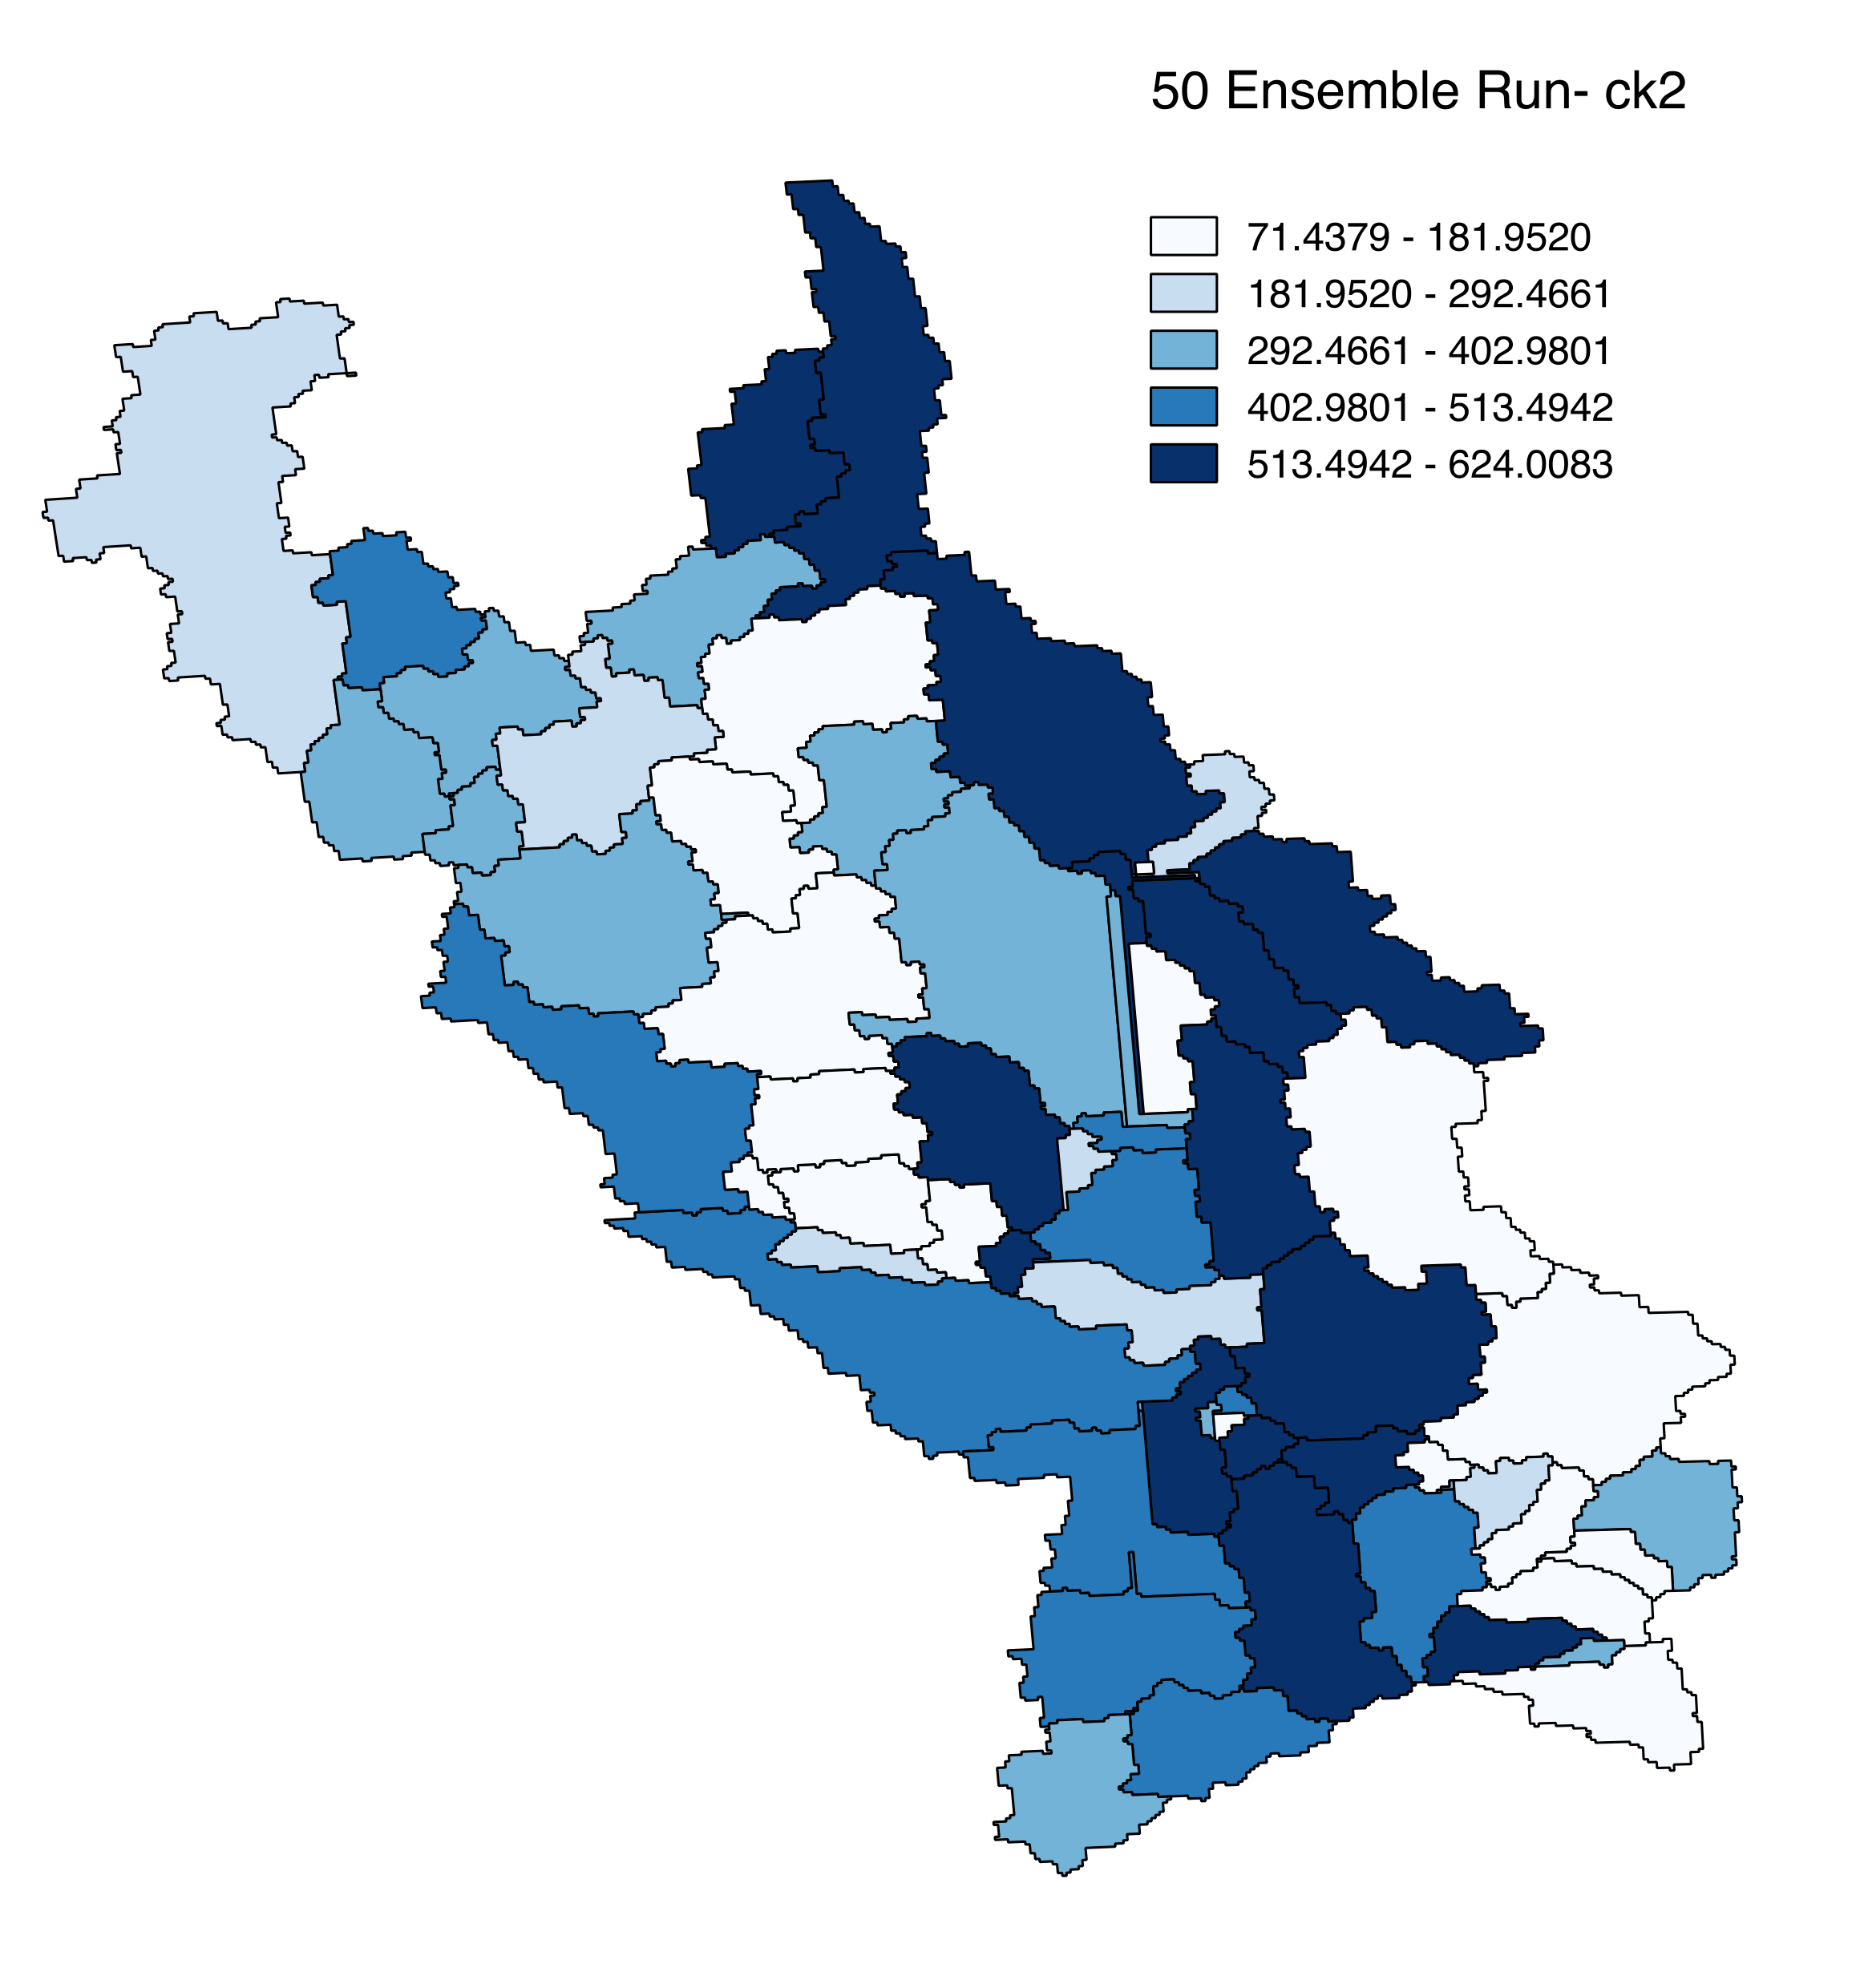
\includegraphics[width = .48\linewidth]{ck250}}\\
\subcaptionbox{100 ensemble run: \texttt{perc}\label{2}}{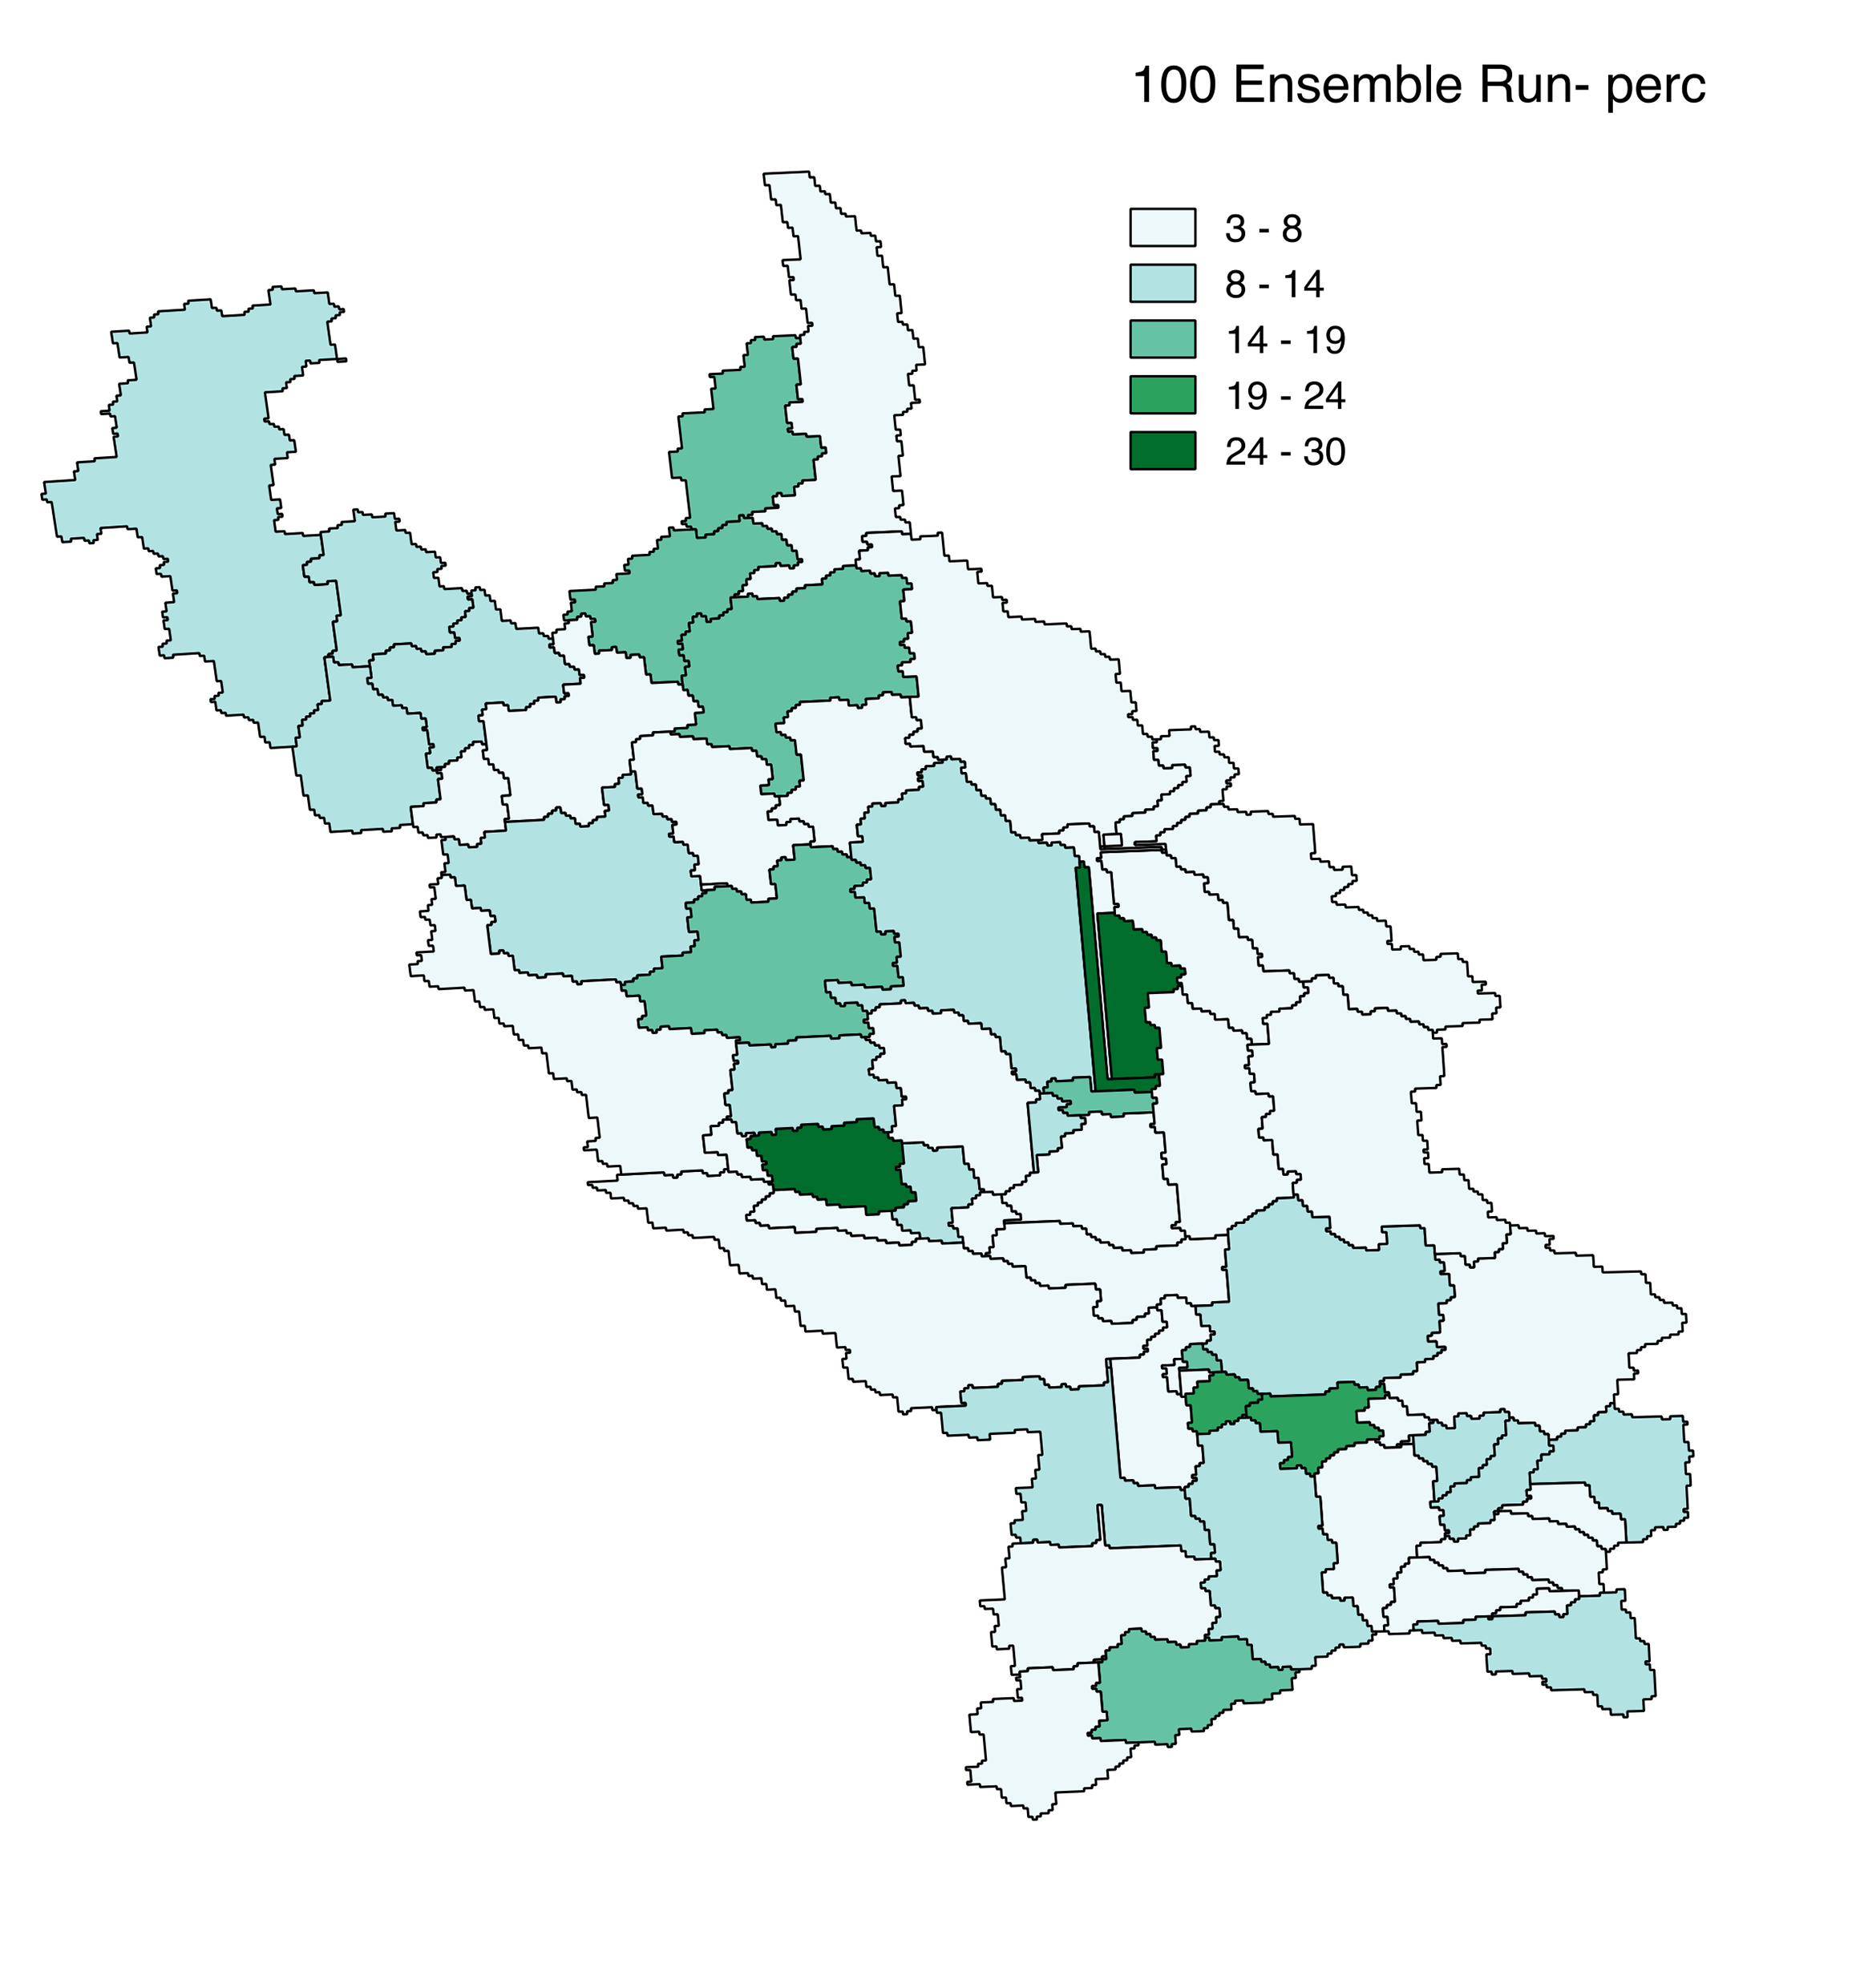
\includegraphics[width = .48\linewidth]{perc100}} &
\subcaptionbox{50 ensemble run: \texttt{perc}\label{2}}{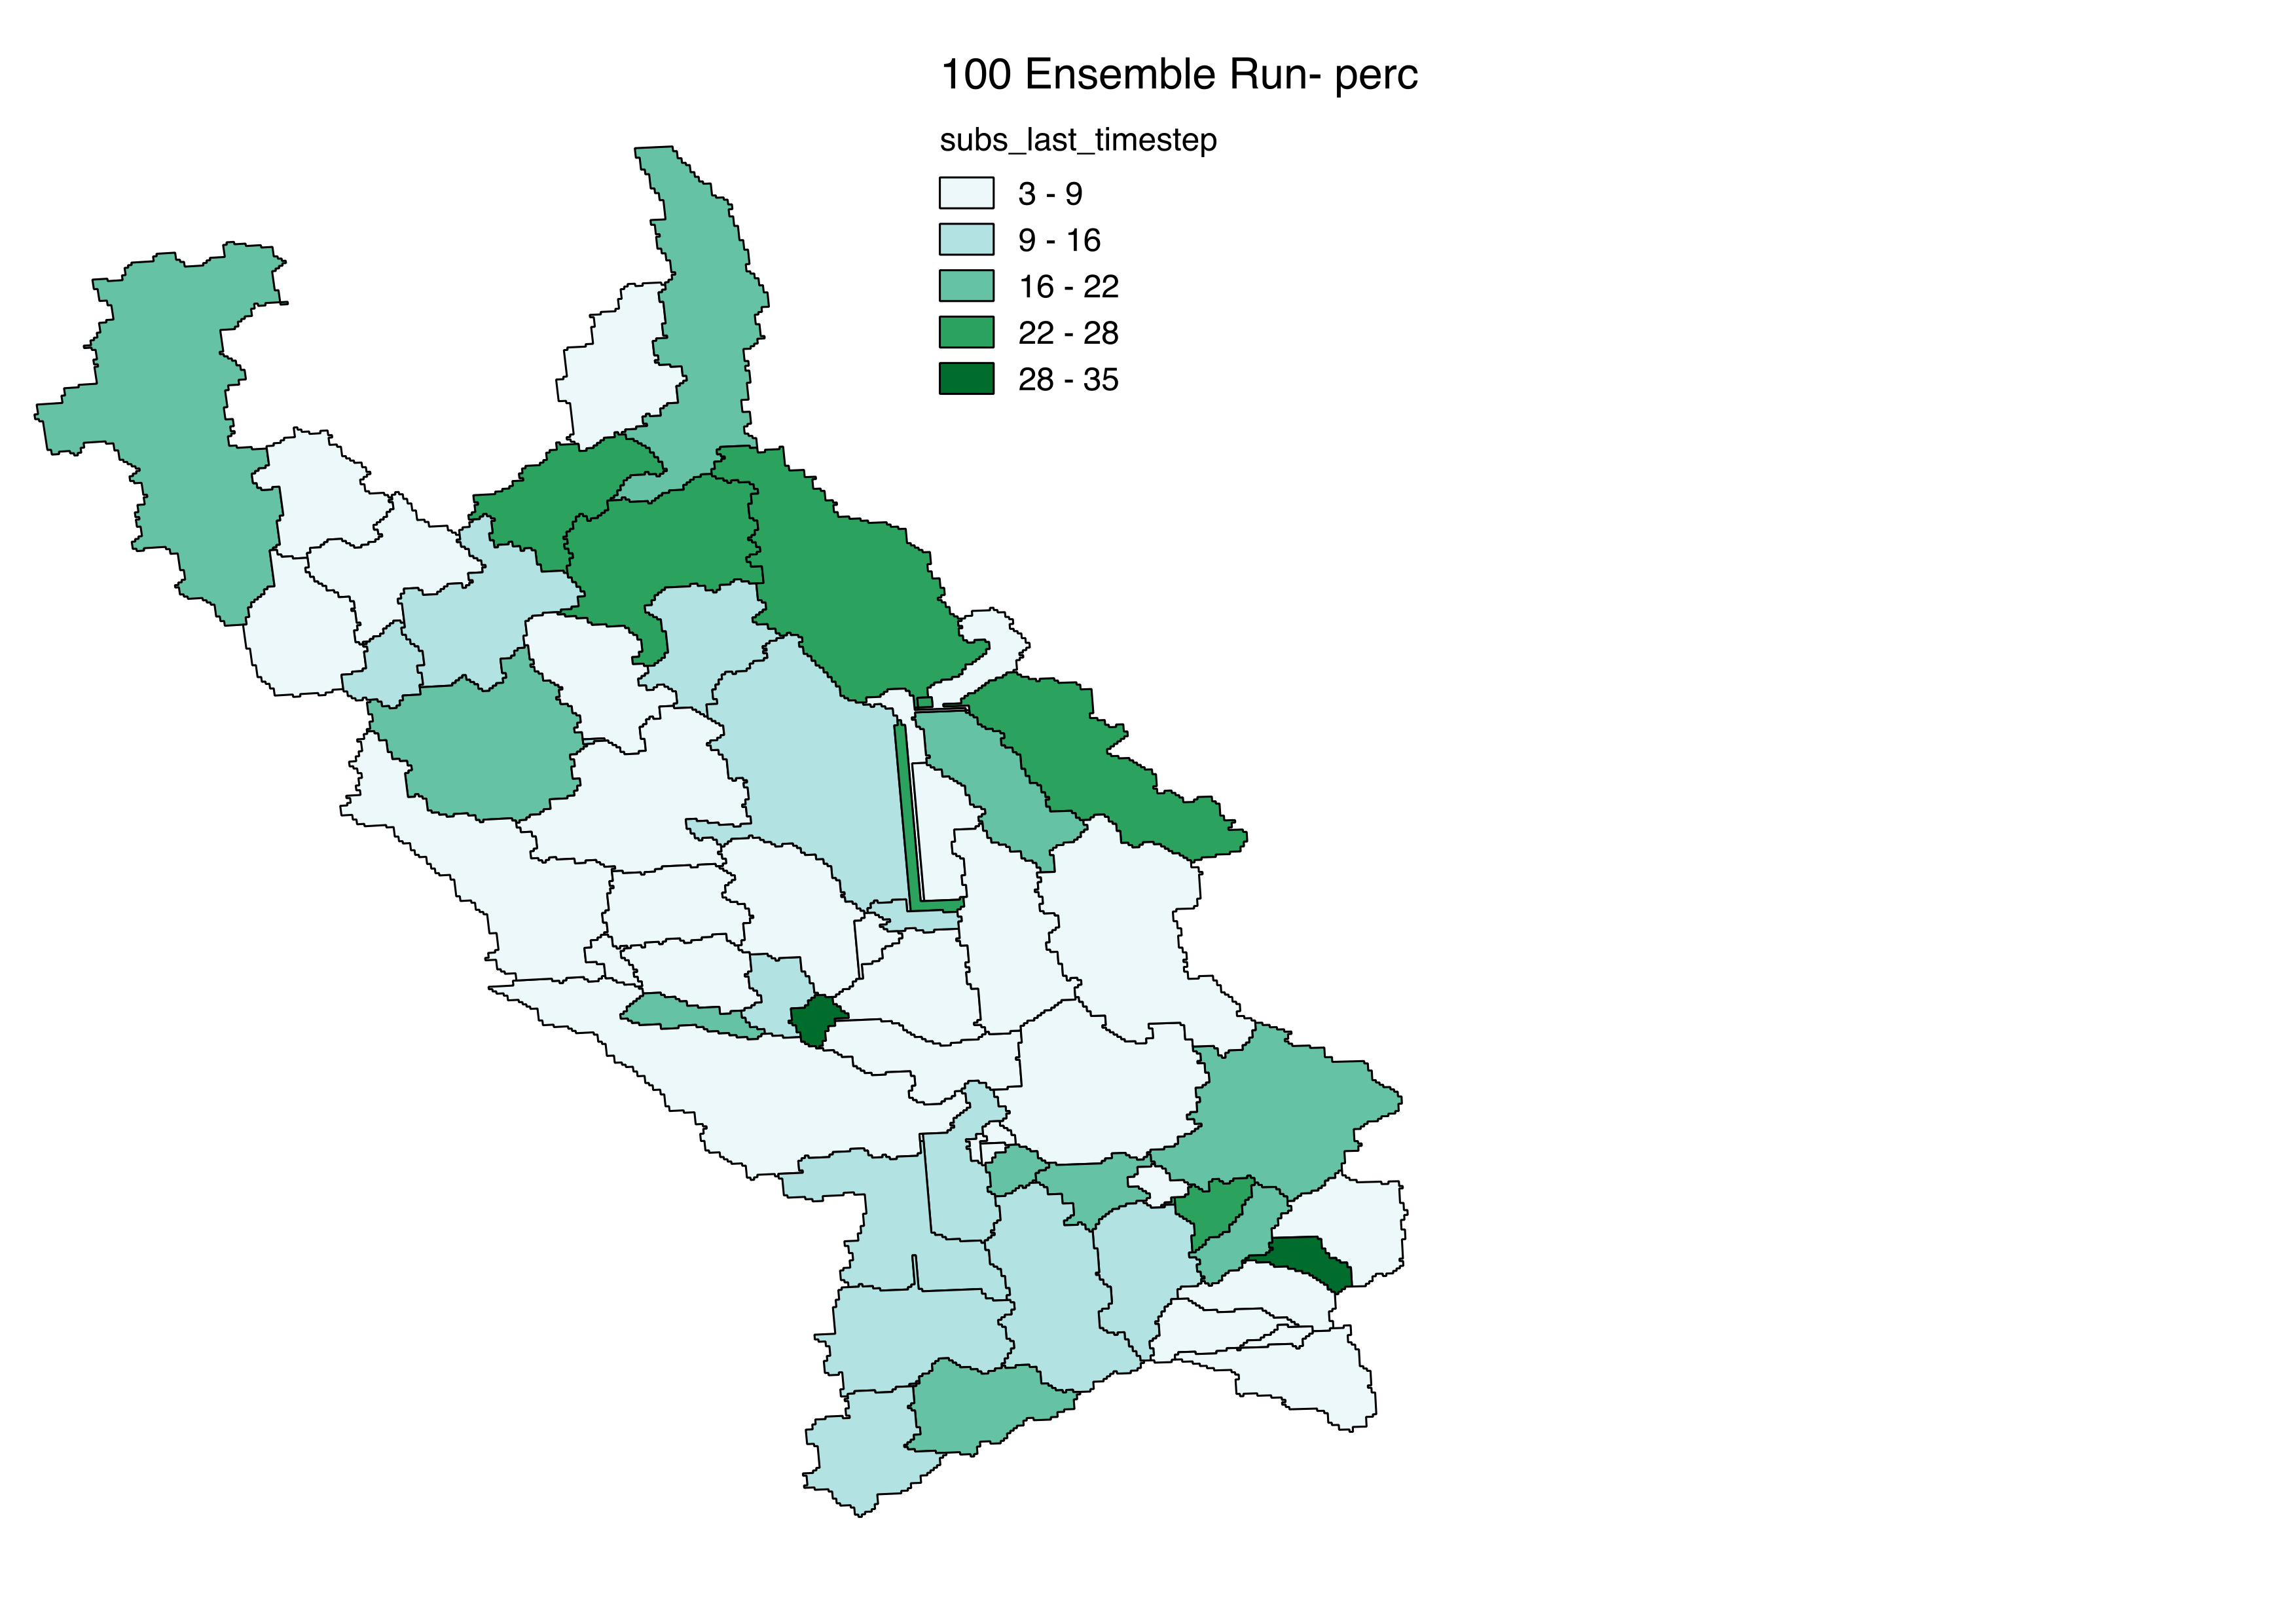
\includegraphics[width = .48\linewidth]{perc50}}

\end{tabular}
\captionof{figure}{Final parameter distributions for the 50 and 100 ensemble runs of the complete dataset}
\label{fig:str_unfiltered_gw}
\end{figure}

\begin{figure}
\begin{tabular}{cc}

\subcaptionbox{Catchment 115\label{2}}{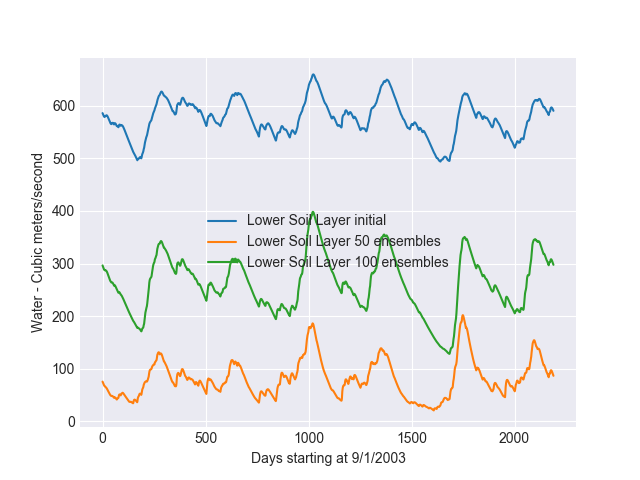
\includegraphics[width = .48\linewidth]{str115gw}} &
\subcaptionbox{Catchment 139\label{2}}{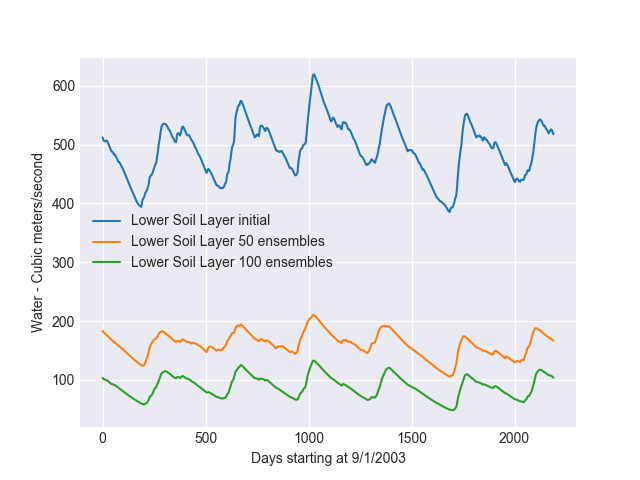
\includegraphics[width = .48\linewidth]{str139gw}}\\
\subcaptionbox{Catchment 165\label{2}}{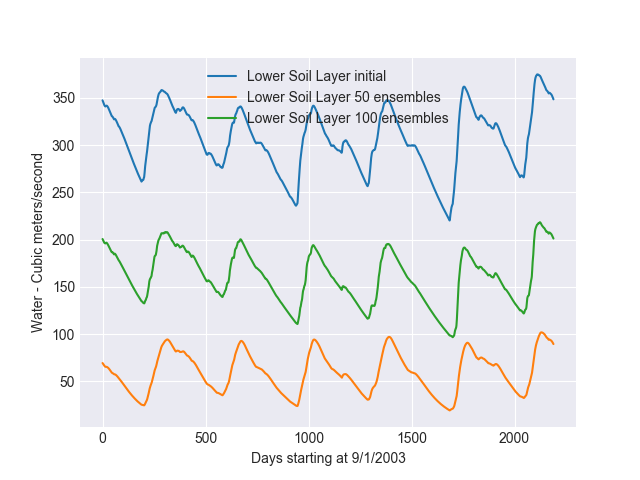
\includegraphics[width = .48\linewidth]{str165gw}} &
\subcaptionbox{Catchment 173\label{2}}{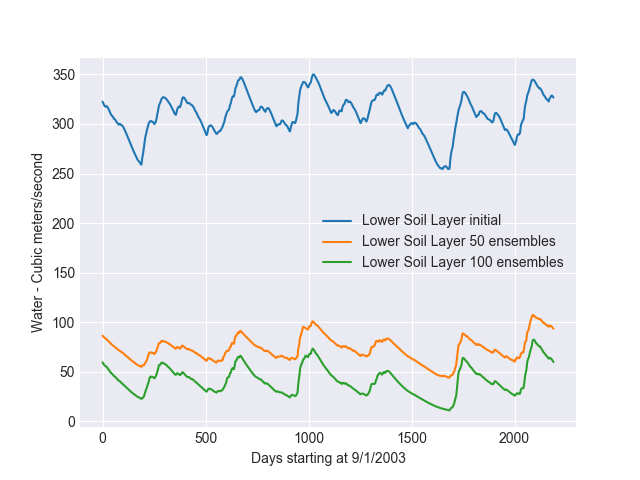
\includegraphics[width = .48\linewidth]{str173gw}}

\end{tabular}
\captionof{figure}{Lower groundwater reservoir water levels from the runs in Figure \ref{fig:str_unfiltered}}
\label{fig:str_unfiltered_gw}
\end{figure}

\subsection{Ensemble Variance}
\label{sec:ensemble-var}
While the Dual State Hierarchical Ensemble Kalman Filtering algorithm possesses many of the same characteristics as the standard Dual State Ensemble Kalman Filtering algorithm developed by Moradkhani et. al in 2005 \cite{Moradkhani2005}, there are some important differences. One of of the largest differences is the DSHenKF's ensembles' tendency to rapidly collapse to the ensemble mean after the mean locks onto a working parameter value. In a standard Ensemble Kalman Filter this variance collapse would be an unwanted effect because the variance between ensembles is a measure of the uncertainty in a parameter. However, the nature of the new hierarchical parameter perturbation scheme encourages this behavior through its dynamic weighting of the ensemble mean as ensembles converge. A large variance in ensemble size, in fact, would indicate a larger reliance on the group mean and would indicate the parameter has not yet found a suitable value (see figure \ref{fig:seeking_param} for an example of this.) Consequently, the uncertainty in an ensemble of parameters in the DSHEnKF method is not necessarily a sign of the lack of variance in a parameter and may simply be the result of a calibrated ensemble of parameters or dormant ensemble of parameters that will reconstitute as soon as the value of the parameter becomes relevant to the model's tracking of the observations.

\begin{figure}[h]
    \centering
    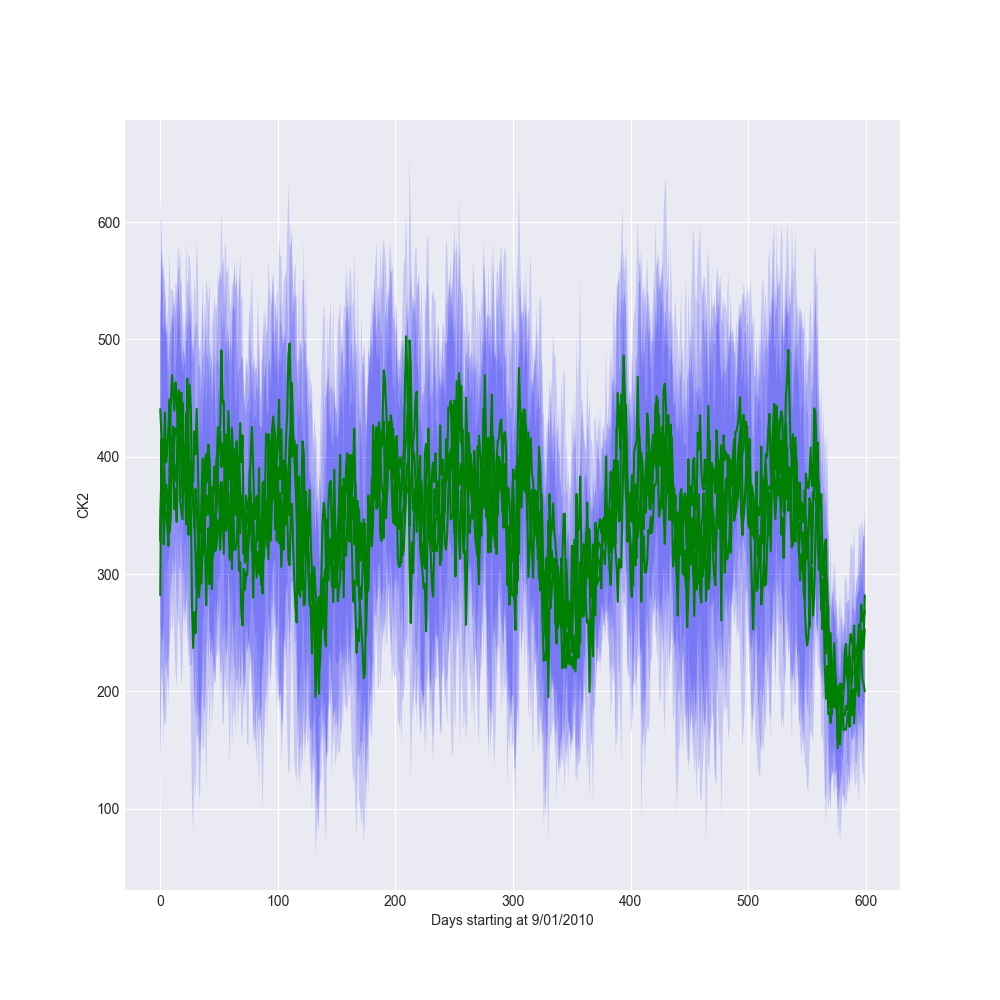
\includegraphics[width=0.95\textwidth]{seeking_param}
    \caption{An example of a parameter's behavior when it is unable to lock onto a a set of values. In this case, this parameter cannot lock because \texttt{b} is too large.}
    \label{fig:seeking_param}
\end{figure}

\section{Further Research Opportunities}

This research introduces and explores the potency of the DSHEnKF method. However, research must be done to compare the accuracy and efficiency of the DSHEnKF method to other filtering algorithms such as the vanilla Dual-State Ensemble Kalman Filter, the Particle Filter, the Joint Ensemble Kalman Filter, and the Unscented Kalman Filter.

Due to computational limitations, certain tests and comparisons such as the optimal ensemble size for the DSHEnKF, the filtering of very large datasets over large time periods, experimentation with multiple hierarchical groupings, or the expansion of state correction to other outputs of the hydrologic model such as groundwater were not attempted. Further research using a different model or more capable computer would flesh out the advantages and disadvantages of the DSHEnKF method.

As discussed in \autoref{sec:ensemble-var}, ensembles collapse quickly in this model. The advantages and disadvantages of this effect should be explored.

Since this study introduced the methodology and results of the DSHEnKF and utilized observed catchments to determine the algorithm's usefulness, further research into the accuracy of the DSHEnKF's ability to calibrate ungaged catchments through its hierarchical component is warranted. The ability to calibrate these ungaged catchments is one of the DSKEnKF's most important applications in the realm of hydrologic modeling.

\section{Summary}
The DSHEnKF method has been proven to be a useful calibration procedure on hierarchically structured datasets, and it has been determined that the DSKEnKF can successfully filter parameters and states and that the final filtered parameters produce more accurate results.  A Dual State Hierarchical Ensemble Kalman Filter was chosen to calibrate the hydrologic model because 1) the DSHEnKF does not have to compute the high dimensional state covariance matrix during the update phase as the ensemble covariance matrix may be substituted in its place, 2) the hydrologic model is a sequential model that could conceivably benefit from real-time parameter correction, and 3) 10+ years of observed streamflow and SWE data may be compared to model data to test for over-fitting. While the potential applications of the DSKEnKF are exciting, further research is needed to understand this method's usefulness when compared to other filtering methods.